\problemname{Minecraftflöde}
Alex gillar vatten. Då är det inte konstigt att hon älskar vatten som forsar. Men det gillar mer än vatten som vatten är vattenfall!
Tänk bara, vatten som forsar i all oändlighet. Hon har hittat en bergvägg som hon tror kommer bli perfekta vattenfallet efter att hon har tillfört lite vatten.
Bergväggen kan modelleras som ett $R \cdot C$ stort rutnät, där $N$ rutor har en klippa som sticker ut. Alex tänkte hälla ut vatten ovanifrån så att det flödar
ner i $K$ stycken kolumner ovanifrån. Vattnet sprider sig enligt följande regler: om rutan under vattnet är tomt sprider den sig dit. Om det finns en klippa ivägen
Sprider den sig istället till höger och vänster. Om det finns en klippa ivägen till höger eller vänster sprider det sig inte i den riktningen. (Notera att detta inte
är exakt hur vatten funkar i Minecraft). Alex har dock svårt att tänka sig hur det kommer se ut, så för att hjälpa henne tänker du skriva ett program som
räknar hur många kolumner som har vatten i sig i botten av klippan.

\section*{illustration av exempelfall 1}
\begin{figure}[!h]
  \centering
  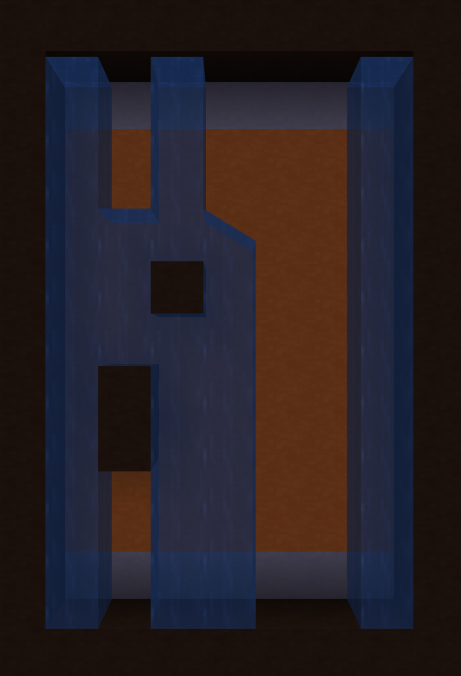
\includegraphics[width=5cm]{flöde.png}
  \quad
  \caption{En illustration av flödet i exempelfall 1. Notera att de gråa delarna ligger utanför klippan och är endast illustrativa.}
\end{figure}

\section*{Indata}
Den första raden innehåller två heltal $R, C$ ($1 \le R, C \le 10^9$), $N$ ($1 \le N \le 10^9$), antalet rader respektive kolumner i fabriken
och antalet saker som ska stoppas in i förslaget.

Därefter följer $R$ rader, som innehåller en sträng $S$ ($|S| = C$). Varje bokstav i denna sträng representerar vilken riktning hoppern på den givna positionen pekar åt.
Varje tecken kommer antingen vara '\texttt{v}' (ner), '\texttt{<}' (vänster), '\texttt{\^}' (upp) eller '\texttt{>}' (höger). Det är garanterat att varje hopper pekar på en annan hopper.

Därefter följer $N$ rader, med två heltal $P_r$ ($0 \le P_r \le R-1$) och $P_c$ ($0 \le P_c \le C-1$), raden och kolumnen som den $i:te$ saken börjar på. 

\section*{Utdata}
Skriv ut $N$ heltal. På den $i:te$ raden, om den $i:te$ saken aldrig krockar, skriv ut "Ingen krock". Annars, skriv ut "Krock vid $r, c$" ($0 \le r \le R-1$, $0 \le c \le C-1$), där 
$r$ och $c$ är raden respektive kolumnen där krocken skedde.

\section*{Poängsättning}
Din lösning kommer att testas på en mängd testfallsgrupper.
För att få poäng för en grupp så måste du klara alla testfall i gruppen.

\noindent
\begin{tabular}{| l | l | p{12cm} |}
  \hline
  \textbf{Grupp} & \textbf{Poäng} & \textbf{Gränser} \\ \hline
  $1$    & $20$      & $R \cdot C \le 1000$ \\ \hline
  $2$    & $30$      & Stenar kan inte röra varandra varken diagonalt, horistonellt eller vertikalt. \\ \hline
  $3$    & $20$      & Stenar kan inte röra varandra diagonalt. \\ \hline
  $4$    & $30$      & Inga ytterligare begräsningar. \\ \hline
\end{tabular}

\section*{Förklaring av exempelfall 1}
TODO (behövs bättre samples + skapa en i minecraft sen)